\begin{circuitikz}[background rectangle/.style={fill=white}, show background rectangle]
        \node(0,0) {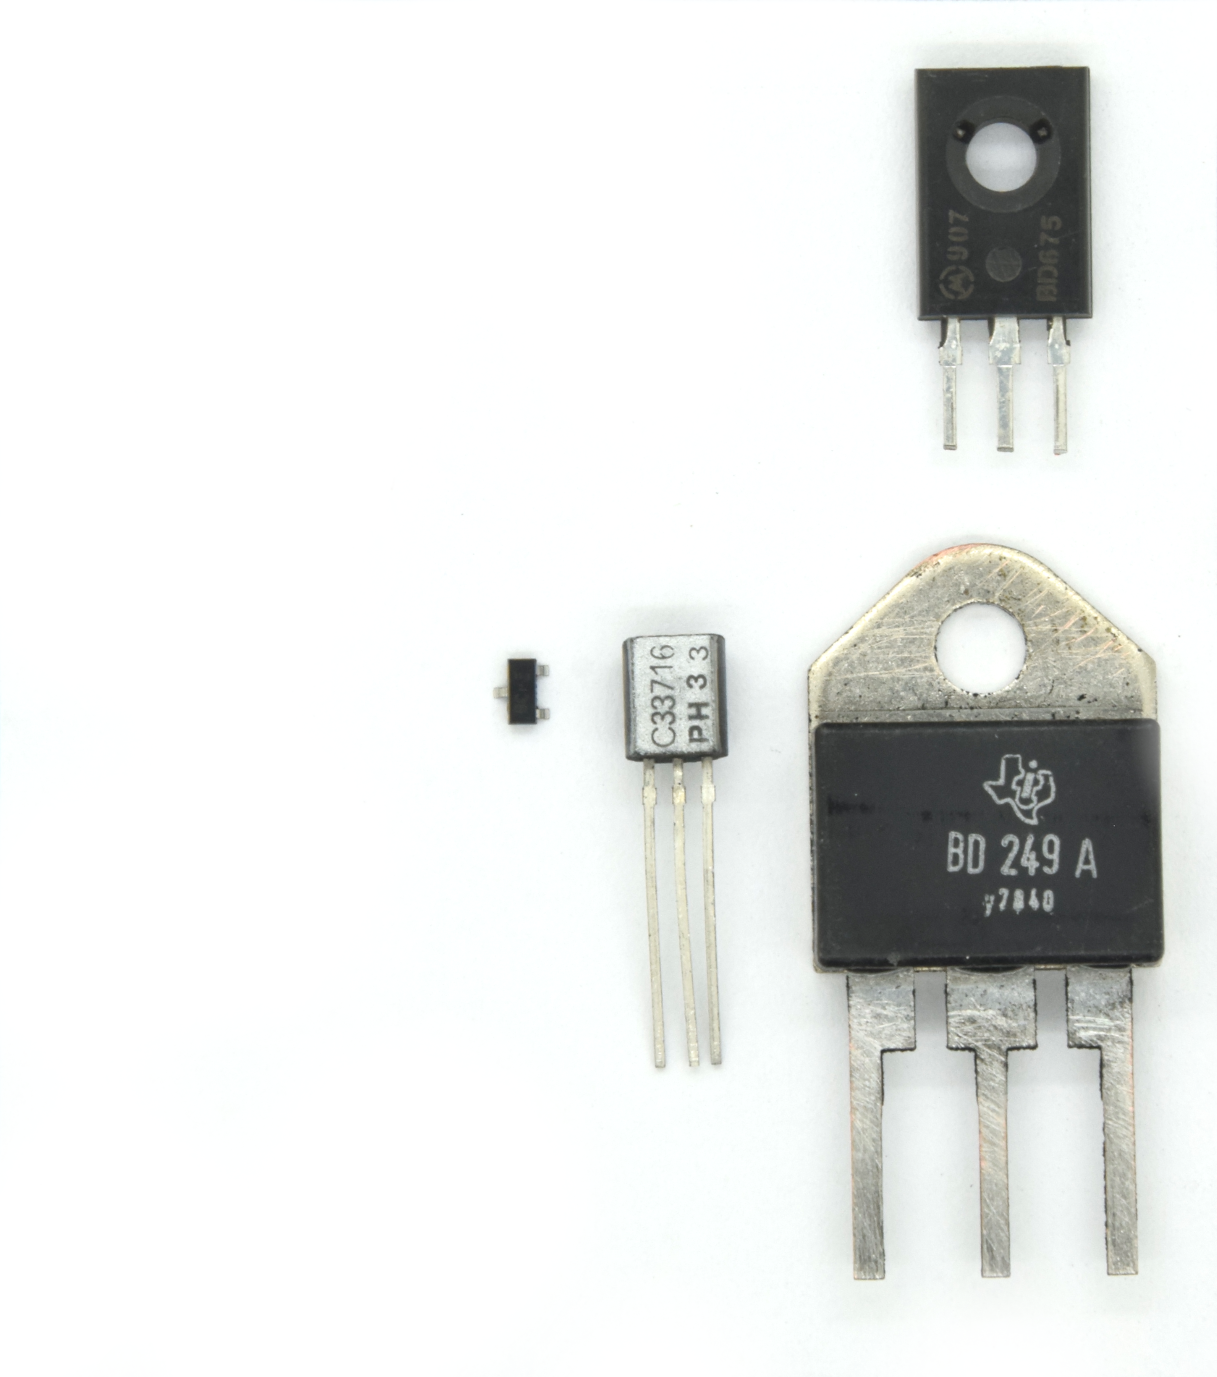
\includegraphics[width=200pt]{foto/10}};
        
        \draw(-2.5,0) node[npn, tr circle]{$T$};
    
        % Beschriftung:
        \draw( 2.15,  1.15) node {\small BD675 \qty{45}{\volt} / \qty{4}{A}};
        \draw( 2.15, -3.75) node {\small BD249A \qty{60}{\volt} / \qty{25}{A}};
        \draw(-0.45,  2.25) node[rotate=90] {\small BCW61C \qty{32}{\volt} / \qty{100}{\milli\ampere}};
        \draw( 0.45,  2.25) node[rotate=90] {\small BC337-16 \qty{45}{\volt} / \qty{800}{\milli\ampere}};
    
        % Pfeile:
        \draw[>=triangle 60, <->] (-1.4,0.675) coordinate(c1) -- ++(0,-1.35) coordinate(c2);
        \draw(c1) -- ++( 0.25,0);
        \draw(c1) -- ++(-0.25,0);
        \draw(c2) -- ++( 0.25,0);
        \draw(c2) -- ++(-0.25,0);
    
        % Text:
        \draw (c1) ++ (0,0.25) node {\qty{1}{\centi\meter}};
\end{circuitikz}